\chapter{Implementation}\label{ch:implementation}

A concrete implementation of applying DRL for robotic grasping with octree-based observations is presented in this chapter. First, design and creation of a simulated RL environment is described, which is then followed by specifics of the utilised RL framework and architecture of CNN for extracting features from octrees of the scene.


\section{Simulation Environment}

As presented in \autoref{sec:rw_reinforcement_learning}, simulations are often used for RL training in order to significantly increase the rate at which data can be collected in a safe manner. In order to implement a virtual setup for training of robotic grasping based on the design from \autoref{ch:problem_formulation}, a simulation must be capable of accurately modelling the physical interactions between a robot and the manipulated objects. Furthermore, it must feature a high fidelity rendering of the scene to provide the required visual observations from viewpoint of a virtual RGB-D camera. Therefore, selection of a robotics simulator is of great importance because it directly influences the robustness of sim-to-real transfer and determines the additional steps that must be taken to achieve such transfer.


\subsection{Selection of Robotics Simulator}

There is a variety of simulation tools that could be applied for training RL agents for robotics, some of which are based on video game engines due to their mature state. Generally, a trade-off between accuracy, stability and performance that must be considered. Although most everyday objects have certain properties of soft bodies, rigid-body dynamics usually provide a satisfactory degree of realism for generic robotic grasping without suffering much performance loss. Therefore, a considered simulator shall have an appropriate physics engine for handling environments with a number of rigid bodies, with support for actuated joints that can be used to connect links of a robot. Similarly, PBR rendering capabilities are highly preferred because of the utilised visual observations. Some of the popular simulators for robotics RL research are therefore described with aim to select one that will be used to implement the environment.

\paragraph{MuJoCo~\protect\cite{todorov_mujoco_2012}} MuJoCo is a physics engine that can accurately model physical interactions. It has been a popular choice for robotics research for years, including RL applications. Unfortunately, MuJoCo is a proprietary software, which has resulted in the decline of its use over the recent years in favour of open-source alternatives. Furthermore, it has limited rendering capabilities.

\paragraph{PyBullet\protect\footnote{\href{https://pybullet.org}{https://pybullet.org}}} PyBullet simulator is built on top of Bullet physics engine, with an experimental support for PhysX\footnote{\href{https://developer.nvidia.com/physx-sdk}{https://developer.nvidia.com/physx-sdk}} back-end. PyBullet is gaining popularity for robotics RL research due to its open-source nature and active development. It provides fast and reliable physical simulations, albeit the available rendering is not photorealistic.

\paragraph{Gazebo Classic~\protect\cite{koenig_design_2004}} Gazebo is one of the oldest open-source robotics simulators and it has a large active user-base because it is the primary simulator for the community of Robot Operating System (ROS) \cite{quigley_ros_2009}. Instead of developing everything from scratch, Gazebo is built on top of already existing physics and rendering engines. By default, it utilises ODE\footnote{\href{https://ode.org}{https://ode.org}} physics engine but others such as DART \cite{lee_dart_2018} and even Bullet are also supported. For rendering, it makes use of OGRE\footnote{\href{https://ogre3d.org}{https://ogre3d.org}}~1 that unfortunately has limited rendering capabilities.

\paragraph{Ignition Gazebo\protect\footnote{\href{https://ignitionrobotics.org}{https://ignitionrobotics.org}}} Due to the limitations and outdated architecture, Gazebo Classic is planned to be deprecated in favour of Ignition Gazebo, i.e.~the next generation of Gazebo. Although it is in its early development, Ignition Gazebo supports DART physics engine and has an upcoming support for Bullet. In addition to OGRE~1, PBR rendering is enabled by using OGRE~2, and there is also a partial support for ray tracing with OptiX\footnote{\href{https://developer.nvidia.com/optix}{https://developer.nvidia.com/optix}}. Both physics and rendering engines can be loaded during runtime due to the utilised plugin-based architecture. Although little RL robotics research has been conducted with the use of Ignition Gazebo so far, \citet{ferigo_gym-ignition_2020} introduced Gym-Ignition as a framework that simplifies its for RL research.

\paragraph{Isaac\protect\footnote{\href{https://developer.nvidia.com/isaac-sim}{https://developer.nvidia.com/isaac-sim}, \href{https://developer.nvidia.com/isaac-gym}{https://developer.nvidia.com/isaac-gym}}} Isaac Sim is a new and promising robotics simulator that is being developed by Nvidia. It utilises PhysX physics engine and has support for state-of-the-art PBR rendering. Isaac Gym is extension of Isaac for RL. One of its significant advantages is that physics computations, rendering as well as the process of determining rewards can be offloaded to GPU and enable running large number of environments in parallel. Unfortunately, the proprietary nature of Isaac might limit its use and possible customisation. Furthermore, Isaac Gym is still available only as an early access as of May~2021 with limited functionalities.

\bigskip

From the considered robotics simulators, Ignition Gazebo is selected in this work due to the following reasons. Compared to MuJoCo that requires a license, it is open-source, which significantly encourages reproducibility. Although Isaac might be a very promising choice for robotics RL research in the future, it is still under development and its proprietary nature could make it difficult to extend for the needs of this work. PyBullet is currently considered to be a one of the best open-source options due to its maturity and a large amount of RL research that has already been conducted with it. However, it lacks PBR rendering capabilities that are already part of Ignition Gazebo. Furthermore, the plugin-based architecture of Ignition Gazebo simplifies addition of new physics engine, where Bullet support is already pending. Its ability to switch between various physics engines during run-time could eventually provide Ignition Gazebo with one of the best physics-based domain randomisation, as it would not only allow randomising the physics parameters but also of the entire physics implementation. The major disadvantage of the selected Ignition Gazebo robotics simulator is its relatively early stage and a very limited amount of RL-specific research conducted with it. Despite of this, the full availability of its source code makes it possible to extend where needed. Gazebo Classic was excluded from this considerations due to its planned deprecation.

Therefore, Ignition Gazebo is used to create an environment for robotic grasping with RL. For the physics engine, the default option of DART is kept unchanged. For rendering engine, OGRE~2 is selected due to its PBR capabilities. Gym-Ignition \cite{ferigo_gym-ignition_2020} is utilised because it simplifies interaction with Ignition Gazebo with focus on RL research. Furthermore, Gym-Ignition facilitates the process of exposing OpenAI Gym interface for the environments, which provides a standardised form that makes environments compatible with most RL frameworks that contain implementations of algorithms.


\subsection{Environment for Robotic Grasping}

In order to create a new RL environment for robotic grasping, several different aspects must be considered and implemented into a single integrated system. This among others includes an accurate model of a robot that needs to be combined with appropriate motion planning and low-level controllers, as well as perception in form of RGB-D frames that can be used for visual observations. Furthermore, a set of 3D object models with appropriate appearance, mechanical and inertial properties is required for training and subsequent evaluation.


\subsubsection{Robot Models}

Support for two articulated robotic manipulators with different kinematic chains and grippers is implemented in order to demonstrate flexibility of the developed environment and applied DRL. This is often neglected from the current robotics RL research, hence it is unknown how well a system reacts to a change of robot, both with respect to the use of same hyperparameters during training and the learned policy itself. These two robots are 6 DOF Universal Robots UR5\footnote{\href{https://universal-robots.com/products/ur5-robot}{https://universal-robots.com/products/ur5-robot}} with OnRobot RG2\footnote{\href{https://onrobot.com/products/rg2-gripper}{https://onrobot.com/products/rg2-gripper}} sweeping-parallel gripper and 7 DOF Franka Emika Panda\footnote{\href{https://franka.de/panda}{https://franka.de/panda}} with its default parallel gripper, both of which are shown in \autoref{fig:simulation_robots}.

\begin{figure}[ht]
    \centering
    \begin{subfigure}[ht]{0.4975\textwidth}
        \centering
        % \includegraphics[width=0.75\textwidth]{implementation/ur5_robot.png}
        \caption*{UR5 with RG2 sweeping-parallel gripper}
    \end{subfigure}%
    ~%
    \begin{subfigure}[ht]{0.4975\textwidth}
        \centering
        % \includegraphics[width=0.75\textwidth]{implementation/panda_robot.png}
        \caption*{Panda with its default parallel gripper}
    \end{subfigure}%
    \caption{Robot models used inside the simulation environment for robotic grasping.}
    \label{fig:simulation_robots}
\end{figure}

Manufacturers of these robots and grippers provide associated 3D CAD models of individual links together with a model of the kinematic chain. However, inertial properties of links and dynamic properties of joints are usually not provided. Therefore, these need to be estimated. In order to do so, inertial properties for both robots and grippers are estimated based on the combination of their documented weight and 3D mesh model, while assuming a uniform density across the bodies. Empirically, it was found that redistributing a portion of hand's mass to each finger provides more stable grasp, which is assumed to be due to the internal mechanical coupling of fingers to the body of hand that is otherwise not accounted for solely from the 3D mesh. For dynamic properties of joints, friction and damping were manually tuned for each joint with aim to achieve a stable manipulation across a variety of control frequencies. Although these estimated values are not based on the real robots, no negative effects for sim-to-real transfer are expected because the action space of DRL agent is in Cartesian space.

With this information, description that uses Simulation Description Format (SDF) compatible with Ignition Gazebo was created for both robots \cite{orsula_manipulators_2021}. A simplification for the sweeping-parallel RG2 gripper was made in order to provide better a stability. It was modelled by using a single actuated revolute joint per finger, whereas the full model would use three additional passive joints on each finger. Parallel gripper for Panda is modelled with two prismatic joints, i.e.~one for each finger.

\paragraph{Motion Planning} To control the motion of both robots, a joint trajectory controller described in \hyperref[app:joint_trajectory_controller]{appendix~\ref*{app:joint_trajectory_controller}} was implemented for Ignition Gazebo. It follows trajectories that are generated in Cartesian space by the use of MoveIt~2\footnote{\href{https://moveit.ros.org}{https://moveit.ros.org}} motion planning framework. In this framework, the default configuration of TRAC-IK \cite{beeson_trac-ik_2015} and RRTConnect \cite{kuffner_rrt-connect_2000} were used for solving kinematics and motion planning, respectively. An advantage of utilising MoveIt~2 is that a single interface can be used to control both simulated and real robots during sim-to-real transfer, however, this feature was not utilised in this work.


\subsubsection{RGB-D Perception}

In order to acquire visual observations from the environment, a virtual RGB-D camera is utilised. Using OGRE~2 rendering engine, it provides aligned RGB image and depth map simultaneously. For both, the resolution is set to~\(256{\times}256\)~px with a field of view (FoV) of~\(52\)\textdegree. Framerate of the camera is set to~\(10\)~Hz. Gaussian noise with~\(\mu{=}0\) and~\(\sigma{=}0.001\) is added to both RGB and depth data in order to slightly increase the realism of observations. The effect of this when compared to real observation is shown in \autoref{fig:rgbd_camera_noise}.

\begin{figure}[ht]
    \centering
    % \includegraphics[width=0.75\textwidth]{implementation/rgbd_noise.pdf}
    \caption{Effect of adding Gaussian noise to RGB-D data in order to improve resemblance to real-world perception.}
    \label{fig:rgbd_camera_noise}
\end{figure}


\subsubsection{Middleware}

ROS~2 is used in this project as a middleware that facilitates communication among the primary nodes of the system, e.g.~RGB-D data stream, requests from motion planner and the simulation environment itself. Whenever data between ROS 2 and the transport layer of Ignition Gazebo is required, a bridge between them is used to convert the messages. The selection of ROS 2 was made because it significantly simplifies the initial research-based development and enables use of helpful libraries and tools for robotics. However, this choice brings a disadvantage for RL because the underlying socket-based transport reduces determinism of the simulation, which prevents exact reproducibility of results even for the same random seed.


\subsubsection{Dataset}

Dataset of scanned objects by \citet{googleresearch_google_2020} was selected for training and evaluation of robotic grasping inside the simulation environment. It is available as a collection from Ignition Fuel, which is a web-based application that allows hosting and sharing of simulation assets. The selected collection contains a thousand of common household objects that are 3D scanned. Their realistic appearance and diverse geometry make them ideal for training of robotic grasping with aim to achieve generalisation. From the dataset,~\(100\) objects shown in \autoref{fig:dataset} were selected and split into training and testing subsets with a ratio of~\(80{/}20\).

\begin{figure}[ht]
    \centering
    \begin{subfigure}[ht]{0.792\textwidth}
        \begin{flushleft}%
            % 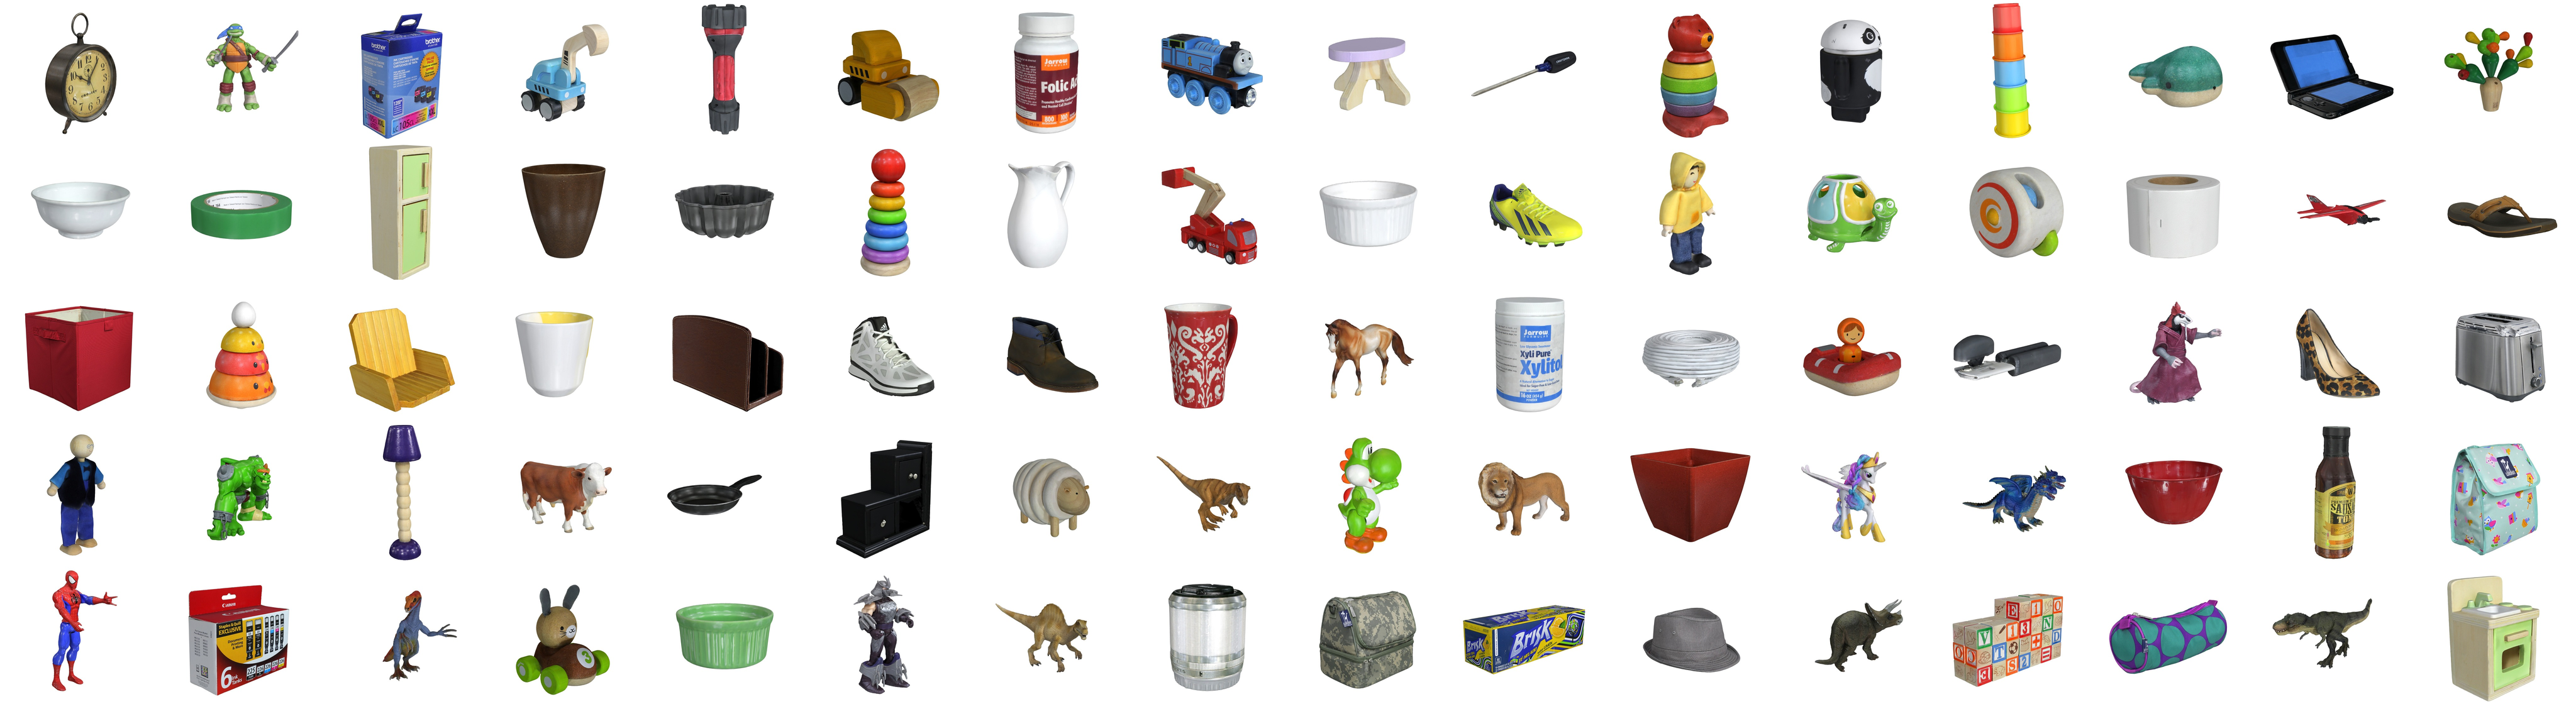
\includegraphics[width=0.995\textwidth]{implementation/training.png}
        \end{flushleft}%
    \end{subfigure}%
    \vrule~%
    \begin{subfigure}[ht]{0.198\textwidth}
        \begin{flushright}%
            % 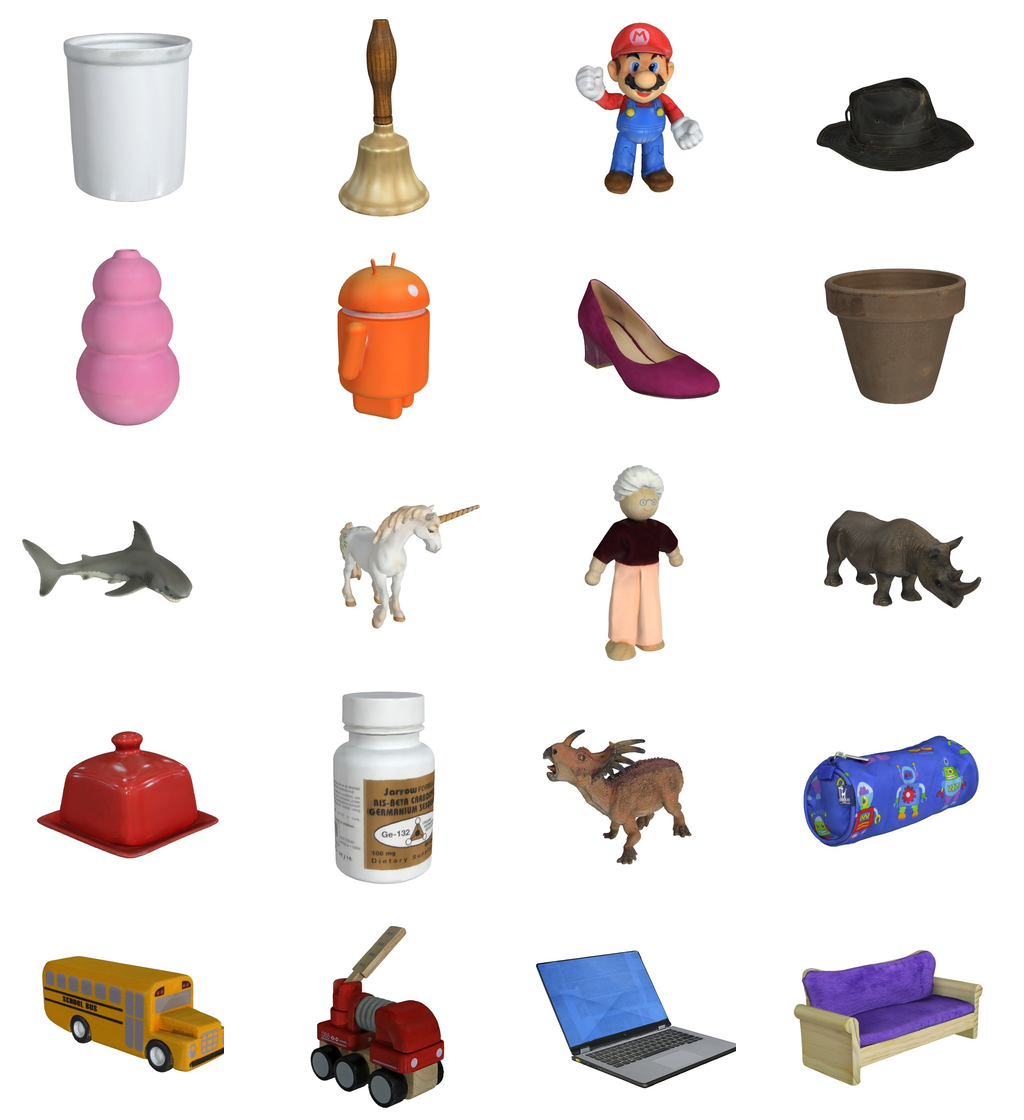
\includegraphics[width=0.995\textwidth]{implementation/testing.png}
        \end{flushright}%
    \end{subfigure}%
    \caption{Training (left) and testing (right) datasets of diverse scanned objects that are utilised in the simulated RL grasping environment. Collection is provided by \citet{googleresearch_google_2020}.}
    \label{fig:dataset}
\end{figure}

All of these objects contain only their corresponding mesh geometry but lack all other properties. Inertial properties were therefore estimated from their geometry in a procedure that is similar to the aforementioned robot models. Mass of each object used during such estimation was randomly selected alongside other properties of the model, which is detailed below in \autoref{sec:impl_domain_randomisation}. This also include the scale of their geometry, as many of these objects would be too large to fit inside the utilised grippers.

The 3D scanned objects contain meshes with a very high resolution, which makes them unsuitable for computing physical interactions due to the enormous computational cost it would bring. Therefore, a low resolution copy of each mesh is created for use as a collision geometry, alongside the original mesh that is kept for visual appearance. Such copy is automatically generated for each model by simplifying the original mesh geometry though decimation procedure based quadric error metrics by \citet{garland_surface_1997}. The algorithm was configured to reduce the geometry to~\(2.5\)\% of the original faces, which was afterward clipped to the range between~\([8,400]\) faces in order to avoid outliers.


\subsubsection{Performance of Simulation}

Having a performant simulation accelerates the data collection, which can in turn enable faster iteration for RL research due to reduced training duration. Besides reducing computational load by decimating geometry of objects, few more tricks are applied in this work.

\paragraph{Disabling of Collision for Robot Links} During early trials, it was found that a collision never occurs between robot links and the environment. This is primarily because MoveIt~2 is used to plan collision-free trajectories. Furthermore the action space is restricted only to the yaw rotation, which further reduces possible collisions. Therefore, collision geometry of robot links is disabled during the training with aim to bring a slight performance gain. The collision geometry of gripper, i.e.~hand and fingers, is kept enabled for both robots as these are required for interaction with the objects.

\paragraph{Larger Simulation Step Size} As previously mentioned, dynamic properties of robot joints were manually tuned in order to obtain stable manipulation across a variety of control frequencies. The primary purpose of this tuning is to allow the use of larger simulation step size, which determines the rate at which simulation progresses. This in turn affects the accuracy of physics as well as the frequency of low-level controller. A step size of~\(4\)~ms is used for the grasping environment because it was found to have a balanced trade-off between physics stability and performance.

With performance in mind, the control rate of RL agent is set to a lower frequency of~\(2.5\)~Hz. This is because the agent only provides high-level control, whereas the motion planner and low-level joint controllers take care of interactions that require faster reaction times.
% TODO: Add RTF (test_env)


\subsection{Domain Randomisation}\label{sec:impl_domain_randomisation}



\subsection{Curriculum and Demonstrations}



\subsection{Sim-to-Real}







\section{Deep Reinforcement Learning}



\subsection{Actor-Critic Algorithms}

\paragraph{Stable Baselines 3}

\paragraph{PyTorch}


\subsection{Feature Extraction}


\subsection{Actor-Critic Network Architecture}


\subsection{Hyperparameter Optimisation}

\paragraph{Optuna}

